\documentclass[aspectratio=169]{beamer}
\usepackage{color,amsmath}
\usepackage{subfigure}
\usepackage{booktabs}
\usepackage{framed}
\usepackage{comment}

\def\vf{\vfill}

%%%%%%%%%%%%%%%%%%%%%%%%%%
\title[]{Preview of next week\\(03-06)}
\author[]{Matthew J. Salganik\\Department of Sociology\\Princeton University}
\date[]{Soc 596: Computational Social Science\\Fall 2016
\vfill
\begin{flushright}
\vspace{0.6in}

\includegraphics[width=0.1\textwidth]{figures/cc.png}
\end{flushright}
}
\begin{document}
%%%%%%%%%%%%%%%%%%%%%%%%%%
\frame{\titlepage}
%%%%%%%%%%%%%%%%%%%%%%%%%%
\begin{frame}

\begin{itemize}
\item Observing behavior
\item Asking questions
\item Running experiments
\item Mass collaboration
\end{itemize}

\end{frame}
%%%%%%%%%%%%%%%%%%%%%%%%%%
\begin{frame}

\begin{itemize}
\item what are experiments?
\item moving beyond simple experiments (and moving beyond MTurk)
\item seeing examples and understanding trade-offs of different approaches
\end{itemize}

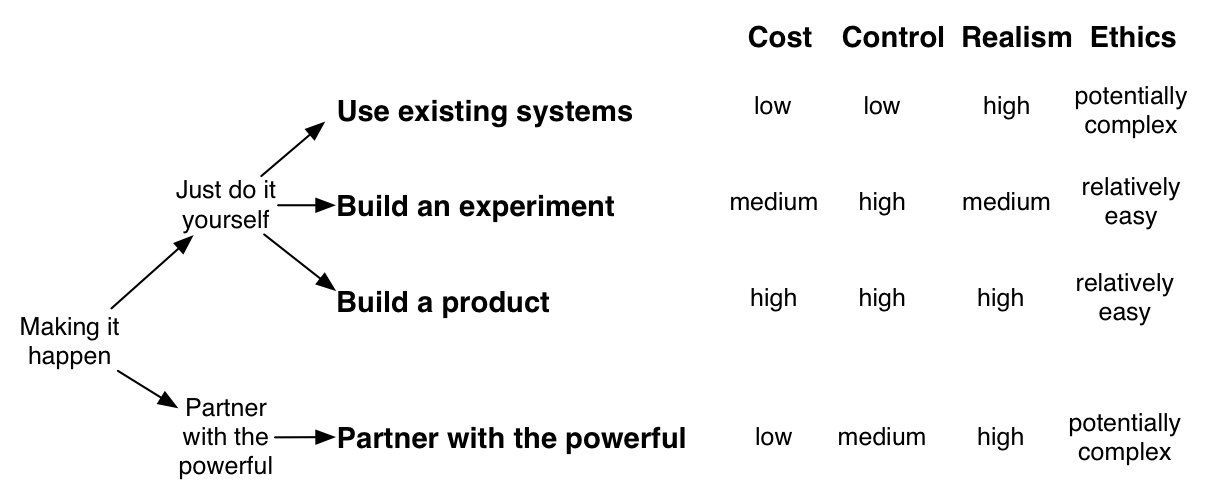
\includegraphics[width=0.7\textwidth]{figures/exp_making_it_happen}


\end{frame}
%%%%%%%%%%%%%%%%%%%%%%%%%%




\end{document}
